\begin{frame}{$"n"$ momentum}
  \label{page:mmN_mom}

  \begin{tabular}{cc}
    \begin{minipage}{0.5\hsize}
      \tiny
      1-stepには過去のデータをインプット済み。\\
      スペックテーターは過去のデータをインプット \cite{ref:d_fermi}\\
      
      $K^- d\rightarrow "n" \pi^{\mp}\Sigma^{\pm}_{forward}$ [下図]は\\
      $d(K^-, n)"\pi^{\mp}\Sigma^{\pm}"$である程度、説明可能\\
      
      $d(K^-, n K^0)"n"$[左図]はバックグラウンドでは足りない。\\
    \end{minipage}
    \begin{minipage}{0.5\hsize}
      \begin{figure}
        $K^0$ tagged \\
        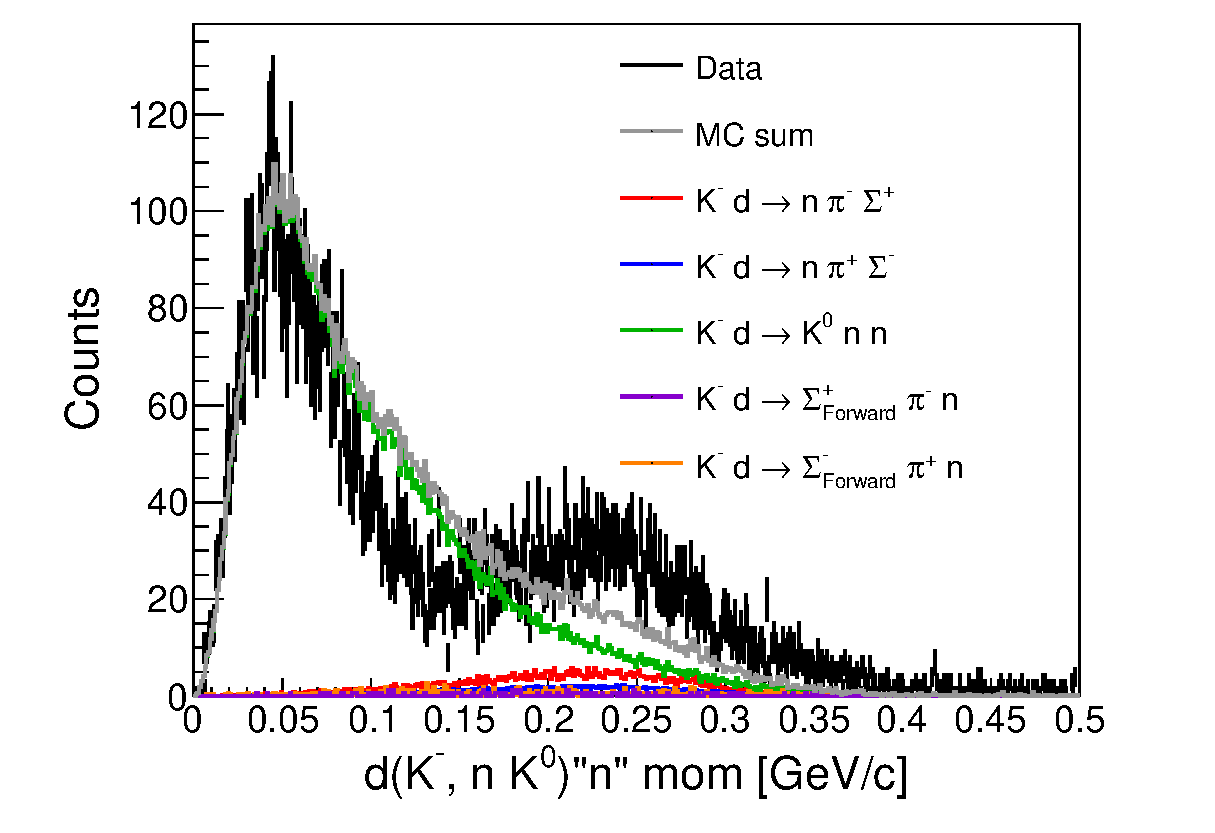
\includegraphics[width=5cm]{../pic/Run78/KN_ana/mmN_mom_K0.eps}
      \end{figure}      
    \end{minipage}
  \end{tabular}

  \begin{tabular}{cc}
    \begin{minipage}{0.5\hsize}
      \begin{figure}
        $\Sigma^+_{forward}$ tagged \\
        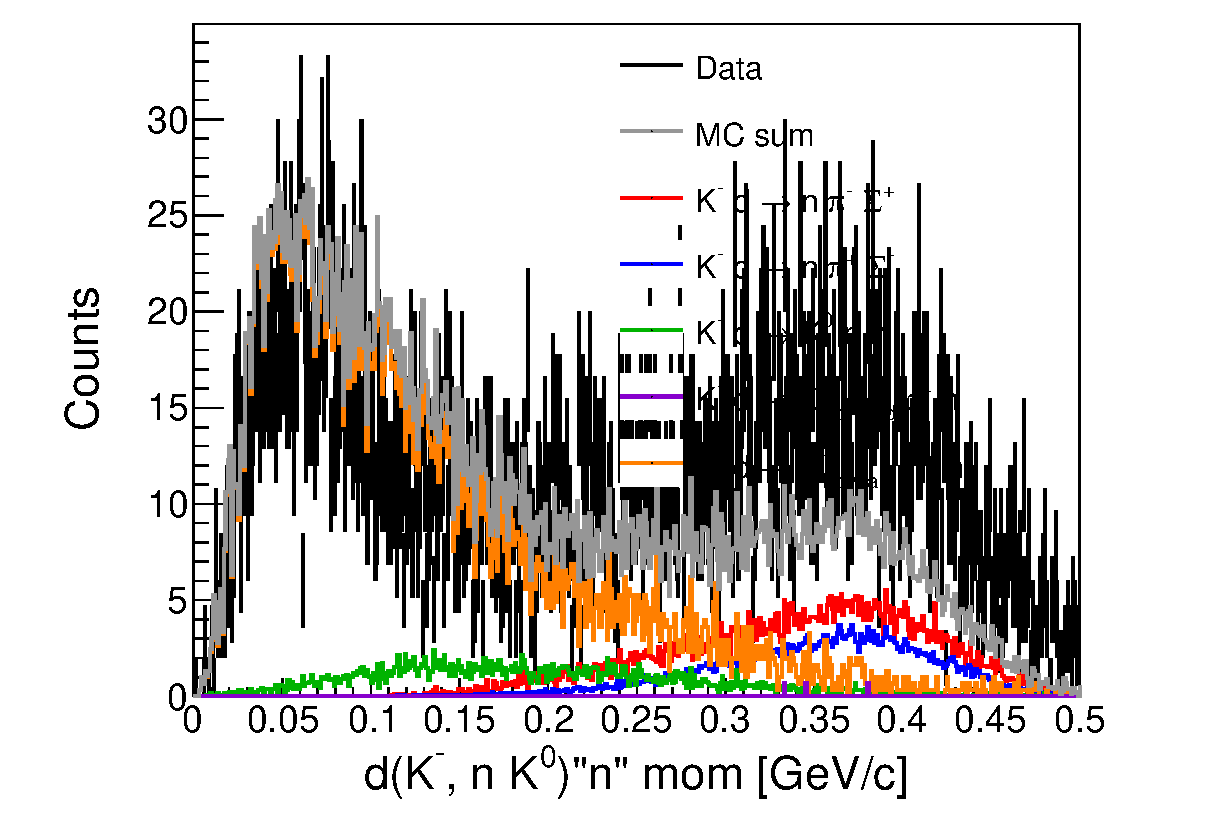
\includegraphics[width=5cm]{../pic/Run78/KN_ana/mmN_mom_Sm.eps}
      \end{figure}
    \end{minipage}
    \begin{minipage}{0.5\hsize}
      \begin{figure}
        $\Sigma^-_{forward}$ tagged \\
        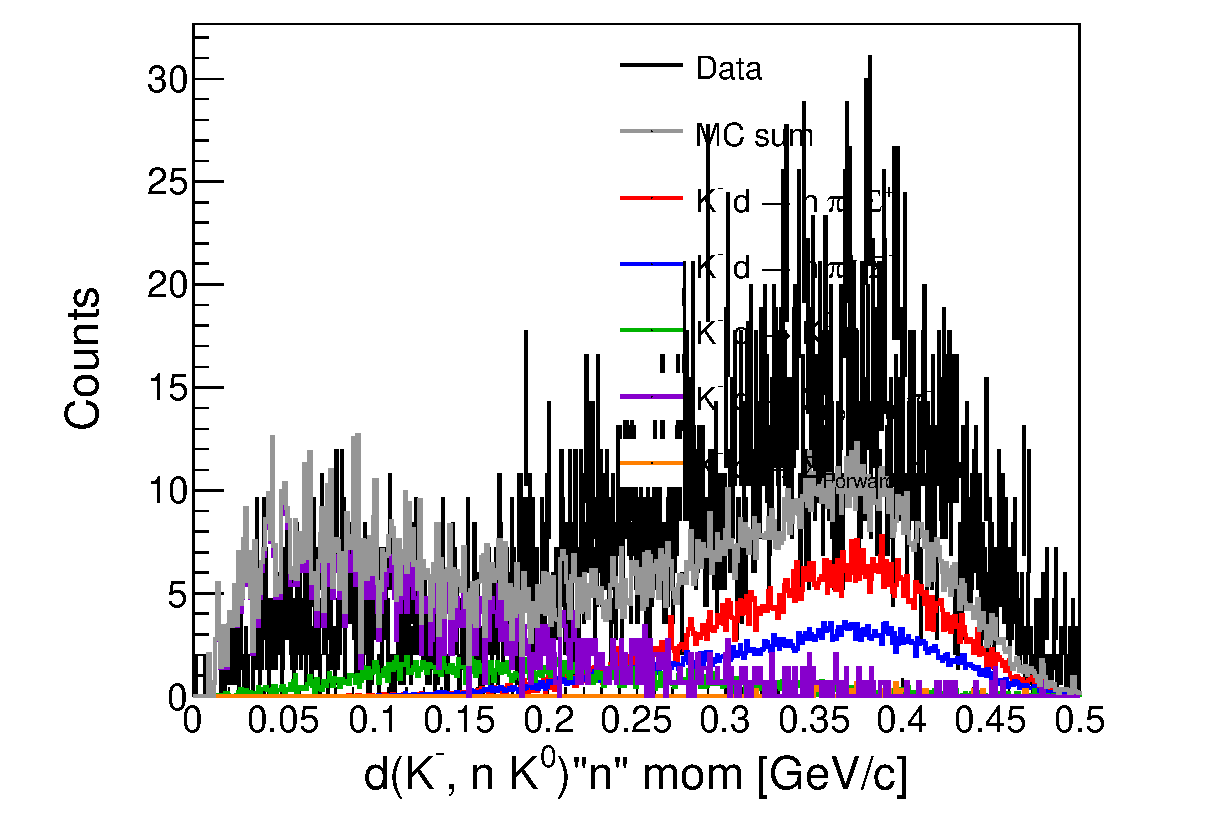
\includegraphics[width=5cm]{../pic/Run78/KN_ana/mmN_mom_Sp.eps}
      \end{figure}
    \end{minipage}
  \end{tabular}
\end{frame}
